%
% 3dimagetemplate.tex
%
% (c) 2021 Prof Dr Andreas Müller, OST Ostschweizer Fachhochschule
%
\documentclass[tikz]{standalone}
\usepackage{times}
\usepackage{amsmath}
\usepackage{txfonts}
\usepackage[utf8]{inputenc}
\usepackage{graphics}
\usetikzlibrary{arrows,intersections,math}
\usepackage{ifthen}
\begin{document}

\newboolean{showgrid}
\setboolean{showgrid}{false}
\def\breite{7}
\def\hoehe{3}

\begin{tikzpicture}[>=latex,thick]

% Povray Bild
\node at (0,0) {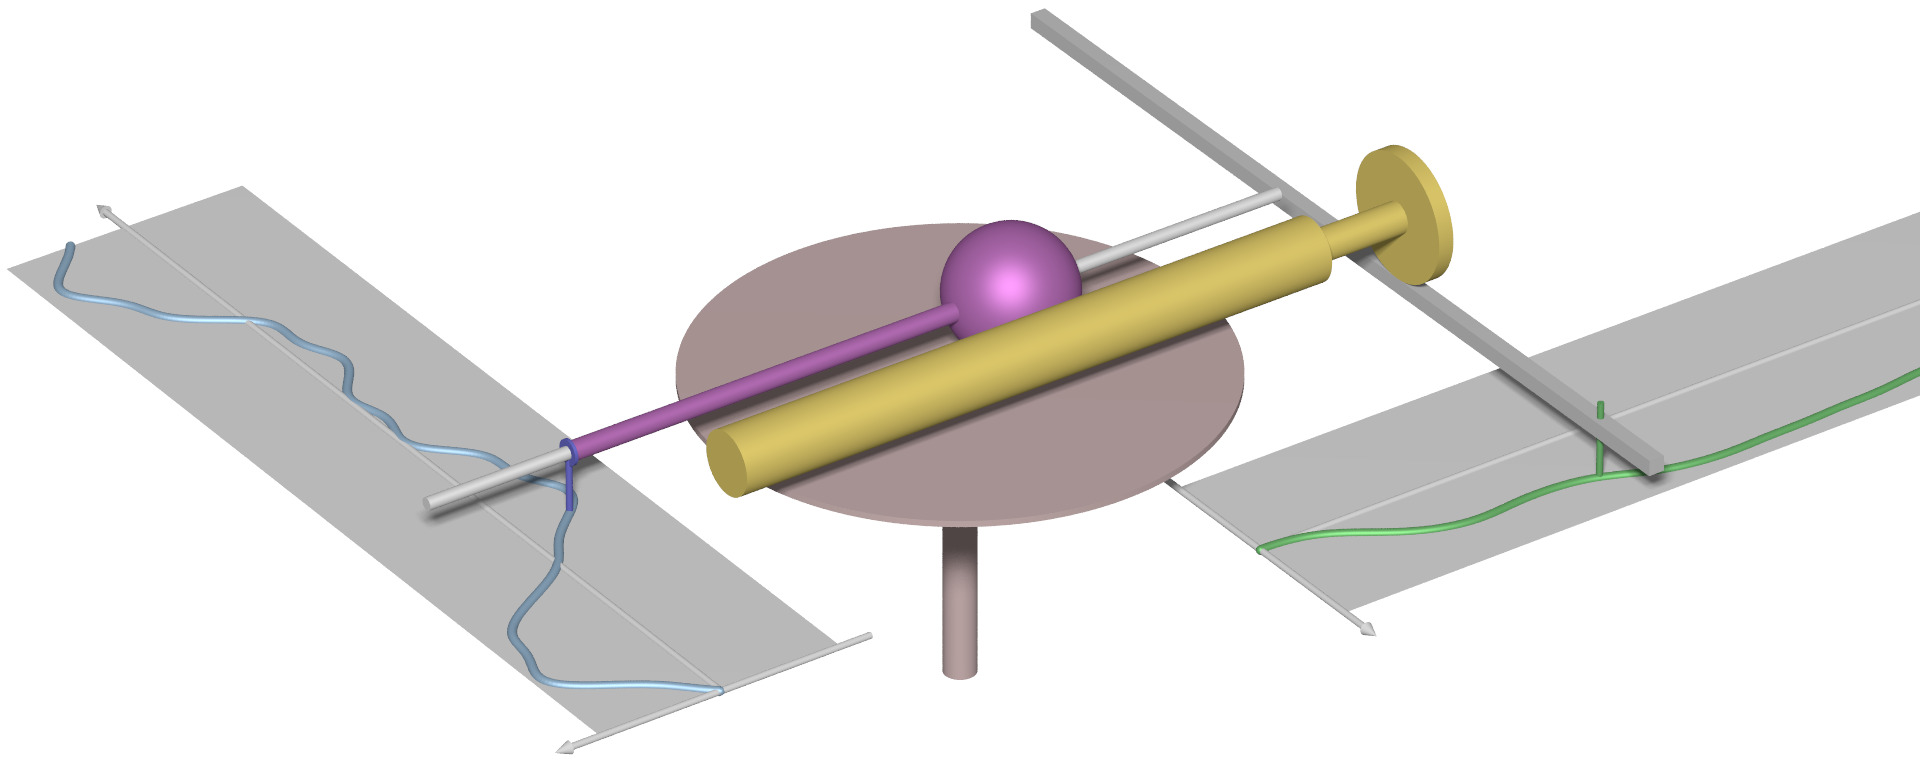
\includegraphics[width=14cm]{ksi.jpg}};

% Gitter
\ifthenelse{\boolean{showgrid}}{
\draw[step=0.1,line width=0.1pt] (-\breite,-\hoehe) grid (\breite, \hoehe);
\draw[step=0.5,line width=0.4pt] (-\breite,-\hoehe) grid (\breite, \hoehe);
\draw                            (-\breite,-\hoehe) grid (\breite, \hoehe);
\fill (0,0) circle[radius=0.05];
}{}

\node at (-6.2,1.4) {$x$};
\definecolor{ffarbe}{rgb}{0.4,0.6,0.8}
\node[color=ffarbe] at (-3.4,-2.5) {$f(x)$};

\definecolor{phifarbe}{rgb}{0.8,0.6,0.6}
\draw[->,color=phifarbe] (0,-2.8) -- (0,-2.3);
\node[color=phifarbe] at (0,-2.60) [right] {$g(x) = \cos\omega x$};

\definecolor{integralfarbe}{rgb}{0.2,0.6,0.2}
\node[color=integralfarbe] at (5.5,-1.5) {$\displaystyle \int f(x) g(x)\,dx$};

\definecolor{spherecolor}{rgb}{0.6,0.2,0.6}
\node at (0.4,1.8) {${\color{ffarbe}f(x)}\cdot {\color{phifarbe}g(x)}$};

\draw[<->,color=spherecolor] 
	(0.1,1.2) to[out=70,in=160]
	(0.4,1.5) to[out=-20,in=110] (0.7,1.1);

\end{tikzpicture}

\end{document}

